\documentclass[answers]{exam}
\renewcommand{\solutiontitle}{\noindent\textbf{}\par\noindent}

\usepackage{fullpage} % Package to use full page
\usepackage{parskip} % Package to tweak paragraph skipping
\usepackage{tikz} % Package for drawing
\usepackage{amsmath}
\usepackage{blindtext}
%\usepackage{hyperref}
\usepackage{graphicx}
\usepackage{enumerate}
\usepackage{caption}
\usepackage{subcaption}
\usepackage{multicol}
\usepackage{mathptmx}
\usepackage{amsmath}
\usepackage{amssymb}
\usepackage{nameref}
\usepackage{minted}
\usepackage{graphicx}

\newcommand{\mypoints}[1]{\textcolor{red}{(#1 points)}}
\newcommand{\myinput}[1]{\textcolor{blue}{#1}}

\title{\normalfont \normalsize
\textsc{{Department of ECE, UCLA \\
ECE 188: Computer Vision}}
\date{\vspace{-12ex}}
}
\begin{document}
\maketitle
\rule{\linewidth}{0.8pt} \\[6pt] 
\noindent
\large\textbf{\textsc{Instructor:}} Prof. Achuta Kadambi, Prof. Stefano Soatto \hfill \large\textbf{\textsc{Name:}} \myinput{Anuj Agrawal}\\
\large\textbf{\textsc{TA:}} Zhen Wang \hfill 
\large\textbf{\textsc{UID:}} \myinput{605627630}
\rule{\linewidth}{0.8pt} \\[6pt] 

\begin{center}
{\textsc{Homework 3}} 
\end{center}
% \vspace{2cm}


\begin{table}[h]
\centering
\resizebox{0.8\textwidth}{!}{%
\begin{tabular}{cccc}
\hline
\multicolumn{1}{c}{\textsc{Problem}} &
\multicolumn{1}{c}{\textsc{Type}} &
\multicolumn{1}{c}{\textsc{Topic}} & \multicolumn{1}{c}{\textsc{Max. Points}} \\  \hline \\ 
 1 & Analytical & Difference of Gaussians & 5 \\ [2mm]
 2 & Analytical & Keypoint Localization for SIFT &  10 \\ [2mm]
 3 & Coding & Image Stitching & 15 \\ [2mm]
 4 & Coding & Olympic Champion using Homography & 5 \\ [2mm]
 5 & Coding & Eight-Point Algorithm & 10 \\ [2mm]
\hline
\end{tabular}
}
\caption*{}
\label{}
\end{table}

\newpage

\section*{Motivation}

In the previous homework and in lecture, we have seen how to extract useful features such as corners using the Harris corner detector and keypoints and feature descriptors using SIFT. These features can then be used to compute correspondences between multiple images, which are useful for a variety of tasks such as image stitching and 3D reconstruction. In this homework, we will focus on SIFT and some applications of correspondences. First, we will examine some analytical aspects of SIFT. We will then transition to various applications of correspondences in 2D: two applications of image stitching, which combines correspondences (extracted via SIFT + RANSAC or manually defined) and homographies. Finally, we will use correspondences and the eight-point algorithm to reconstruct 3D points given correspondences. 

The problem set consists of: 
\begin{itemize}
    \item analytical questions to solidify the concepts covered in the class; and
    \item coding questions to implement some of the algorithms described in class using Python.
\end{itemize}

\section*{Homework Layout}
The homework consists of 5 problems in total, with subparts for each problem. There are 2 types of problems in this homework - analytical and coding. We encourage you to answer all the problems using the Overleaf document; however, handwritten solutions will also be accepted.

\section*{Submission}

You will need to make two submissions: (1) Gradescope: You will submit a PDF with all the answers on Gradescope. (2) CCLE: You will submit your Jupyter notebook (.ipynb file) with filename $\{$your UID$\}$.ipynb with all the cells executed on CCLE. 


\newpage
\section{Difference of Gaussians \mypoints{5.0}}
In class, you were taught that the SIFT (scale-invariant feature transform) detector and descriptor uses Difference of Gaussians (DoG) as a computationally efficient approximation to Laplacian of Gaussians (LoG). In this question, you will derive that the Difference of Gaussians approximates the Laplacian of Gaussians. Let $G(x,y, \sigma) = \dfrac{1}{2\pi \sigma^2} e^{-\big(\dfrac{x^2+y^2}{2\sigma^2}\big)}$ be the 2D Gaussian.

\subsection{Compute $\dfrac{\partial G(x,y,\sigma)}{\partial \sigma}$ \mypoints{1.0}}
Write the expression for $\dfrac{\partial G(x,y,\sigma)}{\partial \sigma}$.
 
\begin{solution}
$\dfrac{\partial G(x,y,\sigma)}{\partial \sigma}$ = $= \dfrac{-1}{\pi \sigma^3}(1- \dfrac{x^2 + y^2}{2\sigma^2})e^{-\big(\dfrac{x^2+y^2}{2\sigma^2}\big)}$
\end{solution}

\subsection{Laplacian of a 2D Gaussian \mypoints{1.0}}
Write the expression for the Laplacian of a 2D Gaussian, $L(x, y)$. \emph{Hint}: this expression was computed in Homework 2.

\begin{solution}
$L(x,y) = -\dfrac{1}{\pi \sigma^4}\big(1 - \dfrac{x^2 + y^2}{2\sigma^2}\big) e^{-\big(\dfrac{x^2+y^2}{2\sigma^2}\big)} $
\end{solution}

\subsection{Relationship of $\dfrac{\partial G(x,y,\sigma)}{\partial \sigma}$ to Laplacian of Gaussian \mypoints{1.0}}
Using the expressions you obtained in the previous two parts, express $\dfrac{\partial G(x,y,\sigma)}{\partial \sigma}$ in terms of the Laplacian of Gaussian $L(x, y)$.
\begin{solution}
$\dfrac{\partial G(x,y,\sigma)}{\partial \sigma}$ = $\sigma L(x,y)$
\end{solution}

\subsection{Approximating $\dfrac{\partial G(x,y,\sigma)}{\partial \sigma}$ \mypoints{1.0}}
Write an expression approximating $\dfrac{\partial G(x,y,\sigma)}{\partial \sigma}$ in terms of $G(x,y,k\sigma)$ and $G(x,y,\sigma)$ for $k \approx 1$.
\begin{solution}
$\dfrac{\partial G(x,y,\sigma)}{\partial \sigma}$ $\approx$ $\dfrac{G(x,y,k\sigma) - G(x,y,\sigma)}{k\sigma - \sigma}$
\end{solution}

\subsection{Approximating Laplacian of Gaussian Using Difference of Gaussians \mypoints{1.0}}
Write an expression approximating the Laplacian of Gaussian, $L(x, y)$, in terms of the Difference of Gaussians, $D(x,y,\sigma)=G(x,y,k\sigma)-G(x,y,\sigma)$, for $k \approx 1$.
\begin{solution}
$\sigma^2L(x,y)$ $\approx$ $\dfrac{G(x,y,k\sigma) - G(x,y,\sigma)}{k - 1}$
\end{solution}

\newpage
\section{Keypoint Localization for SIFT \mypoints{10.0}}
In class, you were taught that SIFT first finds the extrema of the Difference of Gaussians (DoG) and then localizes the keypoints using a Taylor series approximation of the DoG. In this question, you will derive the keypoint localization formula and explain why it is used in SIFT. Let $f(\mathbf{x})$ be the Difference of Gaussians, where $\mathbf{x} = (x, y, \sigma)$ represents the location and scale.

\subsection{Taylor Series Approximation for DoG \mypoints{1.0}}
Write the second order Taylor series approximation of $f(\mathbf{x} + \Delta \mathbf{x})$ centered around $f(\mathbf{x})$. You do not need to compute the derivatives.
\begin{solution}
$f(\mathbf{x} + \Delta \mathbf{x}) = f( \mathbf{x}) + \Delta \mathbf{x}f'( \mathbf{x}) + \dfrac{\Delta \mathbf{x}^2f''( \mathbf{x})}{2} $
\end{solution}

\subsection{Derivative of Taylor Series Approximation \mypoints{1.0}}
Using the Taylor series approximation of $f(\mathbf{x} + \Delta \mathbf{x})$, write the expression for $\dfrac{\partial f(\mathbf{x} + \Delta \mathbf{x})}{\partial \Delta \mathbf{x}}$.
\begin{solution}
$\dfrac{\partial f(\mathbf{x} + \Delta \mathbf{x})}{\partial \Delta \mathbf{x}}$ = $f'(\mathbf{x}) + \Delta \mathbf{x}f''( \mathbf{x}) $
\end{solution}

\subsection{Extrema of Taylor Series Approximation \mypoints{1.0}}
Using the results from the previous part, write the expression for the extrema $\Delta \mathbf{x}$ of the Taylor series approximation.
\begin{solution}
$\Delta \mathbf{x}= \dfrac{-f'(\mathbf{x})}{f''(\mathbf{x})}  = -f''(\mathbf{x})^{-1} f'(\mathbf{x})$
\end{solution}

\subsection{Keypoint Localization \mypoints{1.0}}
\label{keypoint_loc}
Given a keypoint $\mathbf{x} = (x, y, \sigma)$ obtained via the scale-space extrema step of SIFT (lecture 7 slide 40), what is the new keypoint obtained via the Taylor series approximation? Write the expression for the new keypoint.
\begin{solution}
$\mathbf{x}_{new}= \mathbf{x} - f''(\mathbf{x})^{-1} f'(\mathbf{x})$
\end{solution}

\subsection{Purpose of Keypoint Localization \mypoints{3.0}}
What is the purpose of the keypoint localization step in SIFT? Please explain.
\begin{solution}
Scale-space extrema detection produces too many keypoint candidates, some of which are unstable i.e. low contrast or far-off. To refine our search we perform a interpolation to the nearby data for accurate location, scale, and ratio of principal curvature. Localization using extreme detection substantially improves matching and stability. We use this interpolation value to discard far-off and low contrast points and get distinct points.
\end{solution}

\subsection{Inaccuracy of Original Keypoint \mypoints{3.0}}
Assume that the new keypoint from part \ref{keypoint_loc} is closer to a different pixel than it is to the original keypoint $\mathbf{x}$. Then, the original keypoint was not completely accurate. Propose a method to obtain a more accurate estimate of the keypoint. \emph{Note:} A similar method can be applied if the scale of the keypoint is inaccurate (i.e. the keypoint's scale is closer to the scale of a different Gaussian kernel used in computing the Difference of Gaussians).
\begin{solution}
For every keypoint candidate we calculate the offset during keypoint localization step.

If this offset is greater that a threshold (such as 0.5) in any dimension then the point lies closer to another candidate keypoint. In this case, we change the sample keypoint and interpolate about that point. 

Finally we add the offset to the location of the keypoint to get the interpolated estimate of the location at the extrema.
\end{solution}

\newpage

\section{Image Stitching \mypoints{15.0}}
In this question, you will be implementing the image stitching pipeline used to create image panoramas. This pipeline combines SIFT, RANSAC, and homographies to find the homography between a pair of images. After finding the homography between the pair of images, you can use it to stitch the two images together.

\emph{Note:} For extracting SIFT keypoints and features, you should install OpenCV version 4.5.1.48, which can be installed either by running the top cell of the Jupyter notebook or by using the following command: 
\begin{minted}{python}
pip install opencv-contrib-python==4.5.1.48
\end{minted}

\subsection{Obtaining SIFT Keypoints and Descriptors \mypoints{1.0}}
(See the Jupyter notebook). In this sub-part, you will write a function to obtain SIFT keypoints and descriptors for an image. Make sure that your code is within the bounding box.

\begin{solution}
\begin{minted}{python}
def run_sift(image, num_features):
    gray= cv2.cvtColor(image,cv2.COLOR_BGR2GRAY)
    sift = cv2.SIFT_create(nfeatures = num_features)
    kp, des = sift.detectAndCompute(gray,None)
    return kp, des
\end{minted}
\end{solution}

\subsection{Finding Initial Correspondences \mypoints{1.0}}
(See the Jupyter notebook). In this sub-part, you will write a function to obtain an initial set of correspondences by matching SIFT descriptors. Make sure that your code is within the bounding box.

\begin{solution}
\begin{minted}{python}
def d(des1, des2):
    return np.linalg.norm(des1 - des2)


def find_sift_correspondences(kp1, des1, kp2, des2, ratio):
    matching_list = list()
    for i in range(len(kp1)):
        ikey = kp1[i]
        ides = des1[i]
        
        if (d(ides, des2[0]) < d(ides, des2[1])):
            key1 = kp2[0] #1st closest
            ds_key1 = des2[0]
            key2 = kp2[1] #2nd closest
            ds_key2 = des2[1]
        else:
            key1 = kp2[1] #1st closest
            ds_key1 = des2[1]
            key2 = kp2[0] #2nd closest
            ds_key2 = des2[0]
            
        for j in range(2, len(kp2)):
            if d(ides, des2[j]) < d(ides, ds_key1):
                key1 = kp2[j]
                ds_key1 = des2[j]
            if (d(ides, des2[j]) < d(ides, ds_key2)) and \ 
            (d(ides, ds_key1) < d(ides, des2[j])):
                key2 = kp2[j]
                ds_key2 = des2[j]
                
        if d(ides, ds_key1) < ratio * d(ides, ds_key2):
            #matching_list.append([[ ikey, ides], [ key1, ds_key1]])
            matching_list.append([ikey.pt, key1.pt])
            
    return matching_list
                
\end{minted}
\end{solution}

\subsection{Visualizing Initial Correspondences \mypoints{1.0}}
(See the Jupyter notebook). In this sub-part, you will visualize the initial correspondences obtained by matching SIFT descriptors. Copy the saved image from the Jupyter notebook here.

\begin{solution}
\begin{figure}[H]
    \centering
    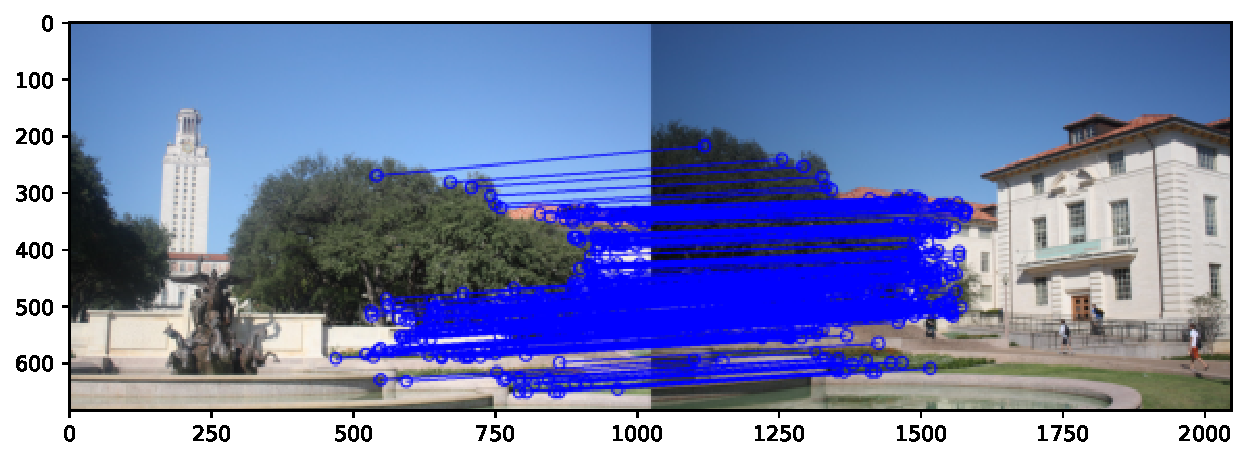
\includegraphics[width=\linewidth]{Images/question_3_3.pdf}
\end{figure}
\end{solution}

\subsection{Computing Homography Using DLT \mypoints{1.0}}
(See the Jupyter notebook). In this sub-part, you will start implementing the RANSAC loop in parts. Write a function to compute a homography between two images given a set of correspondences using direct linear transform (DLT). Make sure that your code is within the bounding box.

\begin{solution}
\begin{minted}{python}
def compute_homography(correspondences):
    A = list()
    for correspondence in correspondences:
        pt1 = correspondence[0]
        pt2 = correspondence[1]
        A.append([-pt1[0], -pt1[1], -1, 0, 0, 0, pt1[0]*pt2[0], \
        pt1[1]*pt2[0], pt2[0]])
        A.append([0, 0, 0, -pt1[0], -pt1[1], -1, pt1[0]*pt2[1], \
        pt1[1]*pt2[1], pt2[1]])
    A_array = np.array(A)
    u, s, vh = np.linalg.svd(A_array, full_matrices=True)
    return vh[-1, :].reshape((3, 3))
\end{minted}
\end{solution}

\subsection{Applying a Homography \mypoints{1.0}}
(See the Jupyter notebook). In this sub-part, you will write a function that applies a homography to warp a set of 2D points. Make sure that your code is within the bounding box.

\begin{solution}
\begin{minted}{python}
def apply_homography(points, homography):
    new_points =[]
    for point in points:
        pt = np.array([[point[0], point[1], 1]])
        pt_t = homography @ (pt.T)
        new_points.append([pt_t[0,0]/pt_t[2,0] , pt_t[1,0]/pt_t[2,0]])
    return new_points

\end{minted}
\end{solution}

\subsection{Computing Inliers \mypoints{1.0}}
(See the Jupyter notebook). In this sub-part, you will write a function that computes the inlier correspondences given a homography, a list of possible correspondences, and a distance threshold. Make sure that your code is within the bounding box.

\begin{solution}
\begin{minted}{python}
def compute_inliers(homography, correspondences, threshold):
    inliers = list()
    outliers = list()
    for correspondence in correspondences:
        pt1 = correspondence[0]
        pt2 = correspondence[1]
        [pt1_new] = apply_homography([pt1], homography)
        if ((pt2[0] - pt1_new[0])**2 + \ 
        (pt2[1] - pt1_new[1])**2)**0.5 < threshold:
            inliers.append(correspondence)
        else:
            outliers.append(correspondence)
            
    return inliers, outliers
    
\end{minted}
\end{solution}

\subsection{RANSAC Loop \mypoints{2.0}}
(See the Jupyter notebook). In this sub-part, you will write a function that implements the RANSAC loop to compute a homography matrix and its inlier and outlier correspondences. This part uses some of the earlier parts such as computing a homography and inliers. Make sure that your code is within the bounding box.

\begin{solution}
\begin{minted}{python}
# Write your code in this cell.

def ransac(correspondences, num_iterations, num_sampled_points, threshold):
    inl_max = []
    outl_max = []
    H_max = 0
    for i in range(num_iterations):
        ransac_corr = random.sample(correspondences, num_iterations)
        H = compute_homography(ransac_corr)
        inl,outl = compute_inliers(H, correspondences, threshold)
        if len(inl_max) < len(inl):
            inl_max = inl
            outl_max = outl
            H_max = H
    return H_max, inl_max, outl_max

\end{minted}
\end{solution}

\subsection{Visualizing RANSAC Inliers and Outliers \mypoints{1.0}}
(See the Jupyter notebook). In this sub-part, you will visualize the inlier and outlier correspondences obtained from running the RANSAC loop on the initial correspondences obtained from matching SIFT features. Copy the saved images from the Jupyter notebook here.

\begin{solution}
\begin{figure}[H]
    \centering
    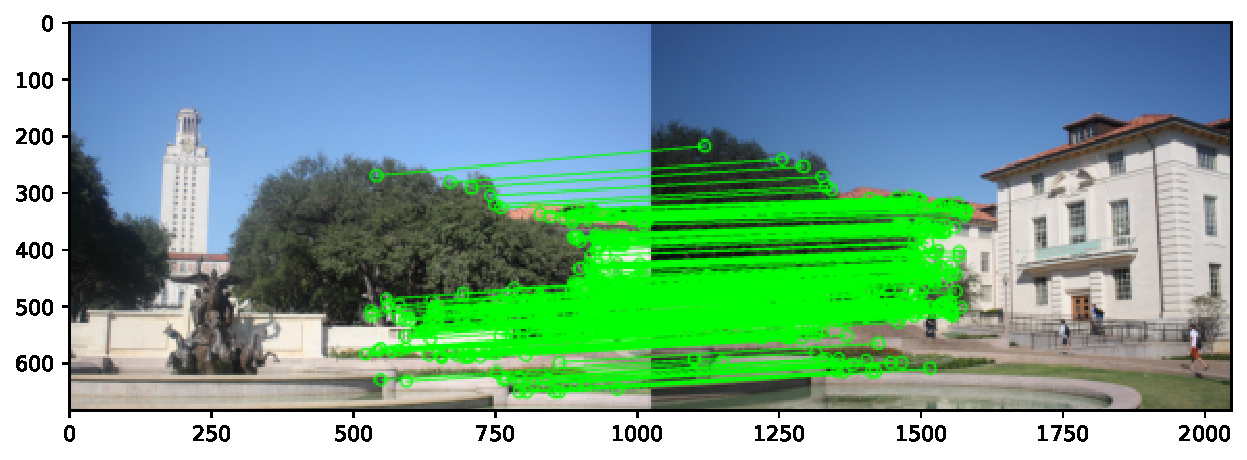
\includegraphics[width=\linewidth]{Images/question_3_8_inliers.pdf}
    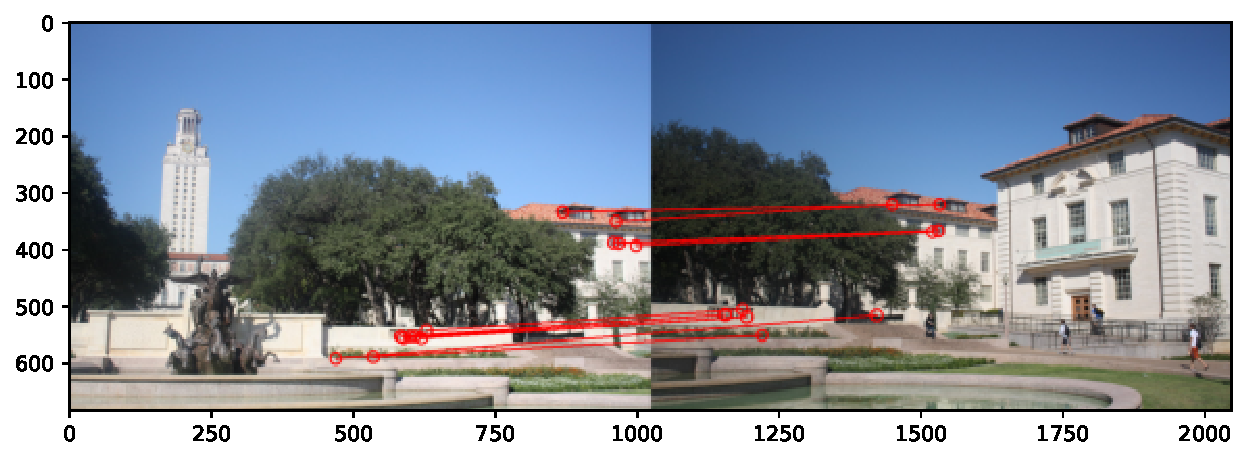
\includegraphics[width=\linewidth]{Images/question_3_8_outliers.pdf}
\end{figure}
\end{solution}

\subsection{Bilinear Interpolation \mypoints{1.0}}
(See the Jupyter notebook). In this sub-part, you will start implementing the actual image stitching in parts. As the image stitching relies on inverse warping and hence, interpolation, write a function that implements bilinear interpolation. Make sure that your code is within the bounding box.

\begin{solution}
\begin{minted}{python}
def interpolate(image, loc):
    x, y = loc[0], loc[1]
    x_int, y_int = int(x), int(y)
    dx, dy = x - x_int, y - y_int
    return (image[x_int,y_int]*(1-dx)*(1-dy)) \ 
    +(image[x_int+1,y_int]*dx*(1-dy))+(image[x_int,y_int+1]*(1-dx)*dy) \ 
    +(image[x_int+1, y_int+1]*dx*dy)
\end{minted}
\end{solution}

\subsection{Image Stitching Given Homography \mypoints{2.0}}
(See the Jupyter notebook). In this sub-part, you will  write a function to implement the actual image stitching using inverse warping given two images and the homography between them. Make sure that your code is within the bounding box.

\begin{solution}
\begin{minted}{python}
def stitch_image_given_H(image1, image2, homography):
    h1, w1, _ = image1.shape
    h2, w2, _ = image2.shape
    
    warped_image = np.zeros((h1, w1 + w2, 3))
    warped_image[:h1,:w1] = image1
    
    for y in range(warped_image.shape[0]):
        for x in range(warped_image.shape[1]):
            p = np.array([x, y, 1])
            p_new = homography @ p.T
            p_new = p_new[:-1]/p_new[-1]

            if (p_new[0] < 0 or p_new[1] < 0 \ 
            or p_new[0] > w2 - 1 or p_new[1] > h2 - 1):
                continue

            if 0 <= y < h1 and 0 <= x < w1:
                warped_image[y][x] = (interpolate(image2, \ 
                (p_new[1], p_new[0])) + warped_image[y][x])/2
            else:
                warped_image[y][x] =interpolate(image2,(p_new[1],p_new[0]))

    return warped_image

\end{minted}
\end{solution}

\subsection{Image Stitching: Putting It All Together \mypoints{1.0}}
(See the Jupyter notebook). In this sub-part, you will put everything together and write a function that implements the whole image stitching pipeline. Make sure that your code is within the bounding box.

\begin{solution}
\begin{minted}{python}
def stitch_image(image1, image2, num_features, 
    sift_ratio, ransac_iter, ransac_sampled_points, 
    inlier_threshold, use_ransac=True):
        kp1, des1 = run_sift(image1, num_features)
        kp2, des2 = run_sift(image2, num_features)
        correspondences = \ 
        find_sift_correspondences(kp1, des1, kp2, des2, sift_ratio)
        if use_ransac:
            _, inliers, outliers = \ 
            ransac(correspondences, ransac_iter,
                    ransac_sampled_points, inlier_threshold)
            h = compute_homography(inliers)
        else:
            h = compute_homography(correspondences)
        
        return stitch_image_given_H(image1, image2, h)
    
        
\end{minted}
\end{solution}

\subsection{Visualizing the Stitched Image \mypoints{1.0}}
(See the Jupyter notebook). In this sub-part, you will visualize the stitched image. Copy the saved image from the Jupyter notebook here.

\begin{solution}
\begin{figure}[H]
    \centering
    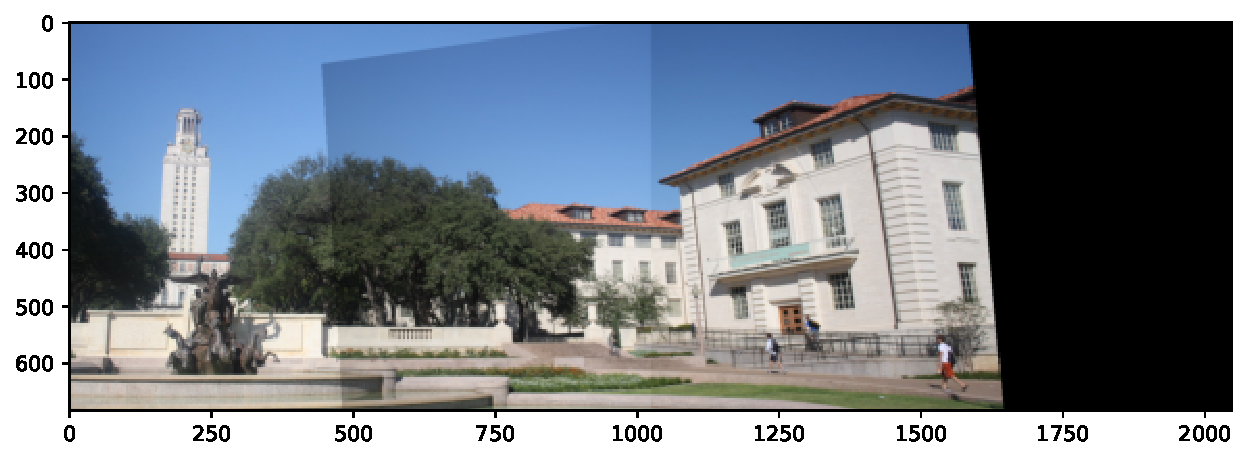
\includegraphics[width=\linewidth]{Images/question_3_12.pdf}
\end{figure}
\end{solution}

\subsection{Visualizing the Stitched Image Without RANSAC \mypoints{1.0}}
(See the Jupyter notebook). In this sub-part, you will visualize the stitched image if you do not use RANSAC. The result here should look much worse than the previous stitched image that uses RANSAC. Copy the saved image from the Jupyter notebook here.

\begin{solution}
\begin{figure}[H]
    \centering
    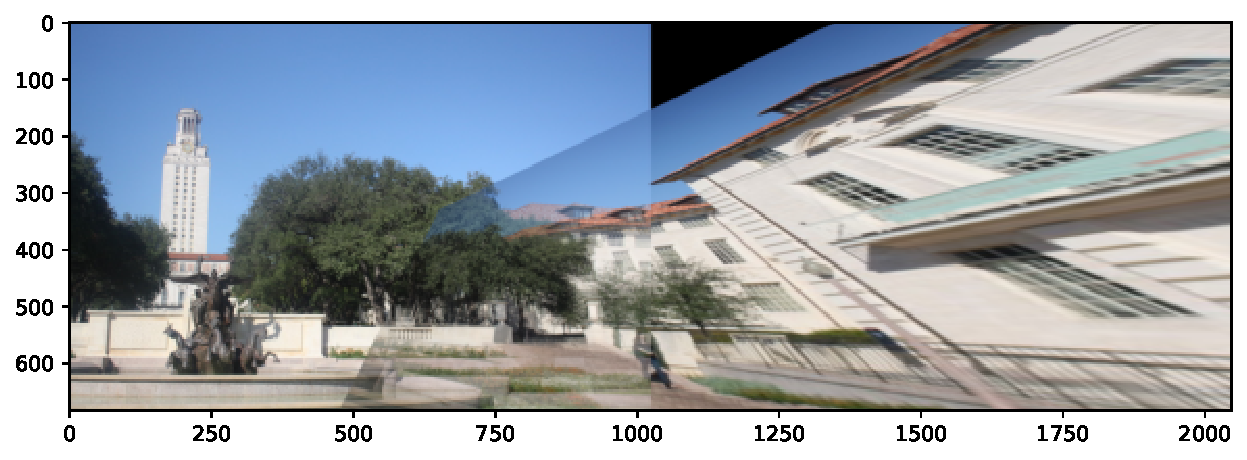
\includegraphics[width=\linewidth]{Images/question_3_13.pdf}
\end{figure}
\end{solution}

\newpage
\section{Olympic Champion using Homography \mypoints{5.0}}

In this question you will make yourself an Olympic swimming champion using homography.

You are given the following image from Olympics 2012, where Gyurta is the new world champion.

\begin{figure}[H]
    \centering
    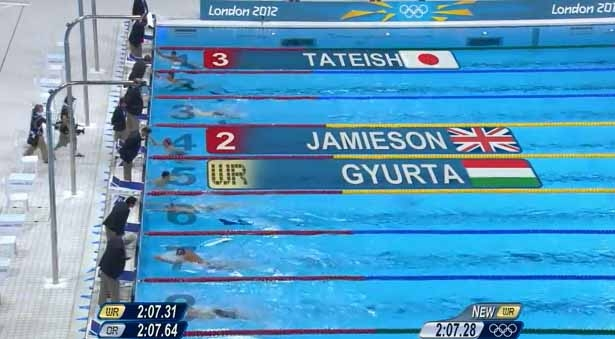
\includegraphics[width=0.9\linewidth]{Images/pool-vfx.jpg}
\end{figure}

You are supposed to use homography and make yourself the new world champion.

\begin{figure}[H]
    \centering
    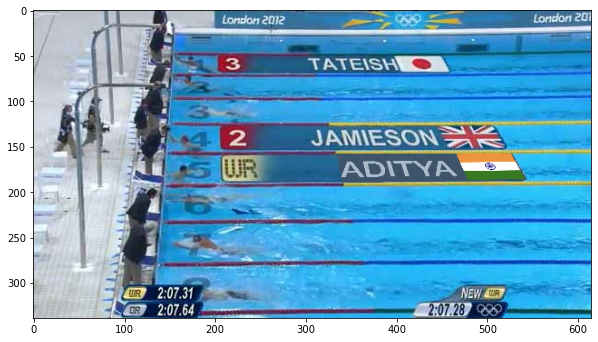
\includegraphics[width=\linewidth]{Images/question_4.png}
\end{figure}

To make yourself the world champion, you will need two images: (1) the Olympic pool, which is given to you and (2) an image with your name and flag besides it. We will provide you with 4 points on the pool image, which will be the corresponding points for the 4 corners of the image (top left, top right, bottom left, bottom right). Using these corresponding points, you will construct the homography matrix and stitch your name on the Olympic record. To get an image with your name and flag, you can use any method of your choice. We used Keynote + Screenshot (for Mac). 

\subsection{Correspondence \mypoints{1.0}}
(See the Jupyter notebook).
Copy the correspondence list from the Jupyter notebook here.
\begin{solution}
\begin{minted}{python}
A_1 = [0, 0]
B_1 = [0, 368]
C_1 = [1650, 0] 
D_1 = [1650, 368]
correspondence = [
                  ([334,158], A_1),
                  ([340,190], B_1),
                  ([528,157], C_1),
                  ([545,187], D_1),
]

\end{minted}
\end{solution}

\subsection{Stitching \mypoints{1.0}}
(See the Jupyter notebook).
In the previous question, you stitched two images side-by-side. In this sub-part, you will stitch one image inside the other. Make sure that your code is within the bounding box.
\textit{Hint}: You will need to use code from the previous question and delete/modify a few lines from it.
\begin{solution}
\begin{minted}{python}
def stitch_image_given_H_new(pool_image, name_flag_image, homography):
    warped = np.copy(pool_image)
    for y in range(warped.shape[0]):
        for x in range(warped.shape[1]):
            p =[x,y]
            [p_new] = apply_homography([p], homography)
            if (p_new[0] < 0 or p_new[1] < 0 \
                or p_new[0] > name_flag_image.shape[1] - 1 \
                or p_new[1] > name_flag_image.shape[0] - 1):
                continue
            warped[y][x] =interpolate(name_flag_image,(p_new[1], p_new[0]))

    return warped
    
\end{minted}

\end{solution}

\subsection{Visualize \mypoints{3.0}}
(See the Jupyter notebook.)
Display the final image with you as the world champion.

\begin{solution}
\begin{figure}[H]
    \centering
    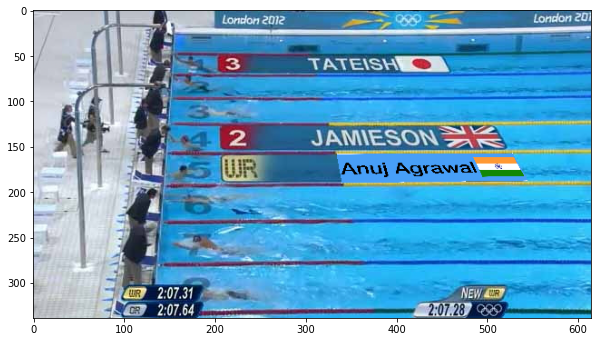
\includegraphics[width=0.9\linewidth]{Images/question_4_Anuj.png}
\end{figure}
\end{solution}

\newpage
\section{Eight-Point Algorithm \mypoints{10.0}}

In this question, you will implement the eight-point algorithm to reconstruct 3D points associated with 2D correspondences of an image pair.

\subsection{Compute the Essential Matrix \mypoints{2.0}}
(See the Jupyter notebook). In this sub-part, you will compute the essential matrix using the eight-point algorithm. Make sure that your code is within the bounding box.
\begin{solution}
\begin{minted}{python}
def compute_essential_matrix(correspondences):
    a = []
    for((x1,y1), (x2,y2)) in correspondences:
        a.append([x1*x2, x1*y2, x1, y1*x2, y1*y2, y1, x2, y2, 1])
        
    A = np.asarray(a)
    vh1 = np.linalg.svd(A)[2][-1]
    Q = np.reshape(vh1, (3,3))
    
    u2, s2, vh2 = np.linalg.svd(Q)
    s_diag = np.diag(s2)
    s_diag[-1,-1] = 0
    Q_mod = (u2 @ s_diag) @ vh2
    return Q_mod
\end{minted}

\end{solution}

\subsection{Compute the Translation and Rotation \mypoints{2.0}}
(See the Jupyter notebook). In this sub-part, you will compute the translation and rotation between the two images' cameras given the essential matrix. Make sure that your code is within the bounding box.
\begin{solution}
\begin{minted}{python}
def compute_translation_rotation(essential_matrix):
    u, s,v = np.linalg.svd(essential_matrix)
    s_diag = np.diag(s)
    mr = np.array([[0, -1, 0],
                     [1, 0, 0],
                     [0, 0, 1]])
    
    R = (u @ mr.T) @ v
    
    T_hat = (u @ mr) @ (s_diag @ u.T)
    T = np.array([T_hat[2,1], T_hat[0,2], T_hat[1,0]])
    
    return T, R, T_hat

\end{minted}
\end{solution}
 
\subsection{Sanity Check Translation and Rotation \mypoints{3.0}}
(See the Jupyter notebook). In this sub-part, you will perform some sanity-checks on the translation and rotation obtained previously. Copy the output from the Jupyter notebook here.
\begin{solution}
\begin{minted}{python}

Translation vector:  [0.71854834 0.00666255 0.02786394]
Rotation matrix: 
 [[ 0.98419658  0.03606853 -0.17336709]
 [ 0.03633853 -0.99933823 -0.0016174 ]
 [-0.1733107  -0.00470807 -0.98485595]]
T_hat: 
 [[ 1.04424451e-05 -2.88351617e-02  6.66254996e-03]
 [ 2.78639384e-02 -6.45670843e-04 -6.94041454e-01]
 [-6.94970171e-03  7.18548338e-01  6.35228398e-04]]
R^T: 
 [[ 0.98419658  0.03633853 -0.1733107 ]
 [ 0.03606853 -0.99933823 -0.00470807]
 [-0.17336709 -0.0016174  -0.98485595]]
R^-1: 
 [[ 0.98419658  0.03633853 -0.1733107 ]
 [ 0.03606853 -0.99933823 -0.00470807]
 [-0.17336709 -0.0016174  -0.98485595]]
\end{minted}
\end{solution}

\subsection{Compute Depths \mypoints{1.0}}
(See the Jupyter notebook). In this sub-part, you will compute the depths of the 3D points corresponding to the given 2D correspondences. Make sure that your code is within the bounding box.

\begin{solution}
\begin{minted}{python}

def compute_depths(correspondences, translation, rotation):
    dpt = []
    for c in correspondences:
        x1 = np.array([*c[0],1])
        x2 = np.array([*c[1],1])
        dpt.append((np.linalg.pinv(np.array([-rotation @ x1, x2]).T)) \ 
        @ translation)
        
    return dpt
    
\end{minted}
\end{solution}

\subsection{Reconstruct 3D Points \mypoints{1.0}}
(See the Jupyter notebook). In this sub-part, you will reconstruct the 3D points given the 2D correspondences and the associated depths. Make sure that your code is within the bounding box.

\begin{solution}
\begin{minted}{python}

def reconstruct_3d(correspondences, depths):
    pts = []
    for i in range(len(correspondences)):
        c = correspondences[i]
        d = depths[i]
        x1 = np.array([*c[0], 1]) * d[0]
        x2 = np.array([*c[0], 1]) * d[1]
        pts.append([x1,x1])
    return pts
    
\end{minted}
\end{solution}

\subsection{Check the 3D Points \mypoints{1.0}}
(See the Jupyter notebook). In this sub-part, you will check the reconstructed 3D points from the first image by reprojecting them into the second image. Copy the output from the Jupyter notebook here.
\begin{solution}
0.027920314207773998
\end{solution}

\end{document}